\documentclass{article}

\usepackage{polski}
\usepackage{setspace}
\usepackage[polish]{babel}
\usepackage[utf8]{inputenc}

\usepackage{graphicx}
\graphicspath{ {./img/} }

\usepackage{menukeys}

\newcommand*\keystroke[1]{%
  \tikz[baseline=(key.base)]
    \node[%
      draw,
      fill=white,
      drop shadow={shadow xshift=0.25ex,shadow yshift=-0.25ex,fill=black,opacity=0.75},
      rectangle,
      rounded corners=2pt,
      inner sep=1pt,
      line width=0.5pt,
      font=\scriptsize\sffamily
    ](key) {#1\strut}
  ;
}

\setlength\parindent{0pt}

\newenvironment{tightlist}{
\begin{itemize}
  \setlength{\itemsep}{1pt}
  \setlength{\parskip}{0pt}
  \setlength{\parsep}{0pt}}
{\end{itemize}}


\author{
	Mateusz Czajka\\
		\texttt{106596}
	\and
		Adam Szczepański\\
		\texttt{106593}
}
\title{Komunikacja Człowiek-komputer\\PONG}

\begin{document}

\maketitle

\section{Wstęp}

Gra Pong powstała jako projekt w ramach przedmiotu Komunikacja Człowiek-Komputer. W rozgrywce uczestniczy dwóch graczy, każdy na własnym komputerze.
Zaprojektowaliśmy minimalistyczny interfejs graficzny, widoczne są jedynie platformy graczy i piłka.

\begin{figure}[!ht]
\centering
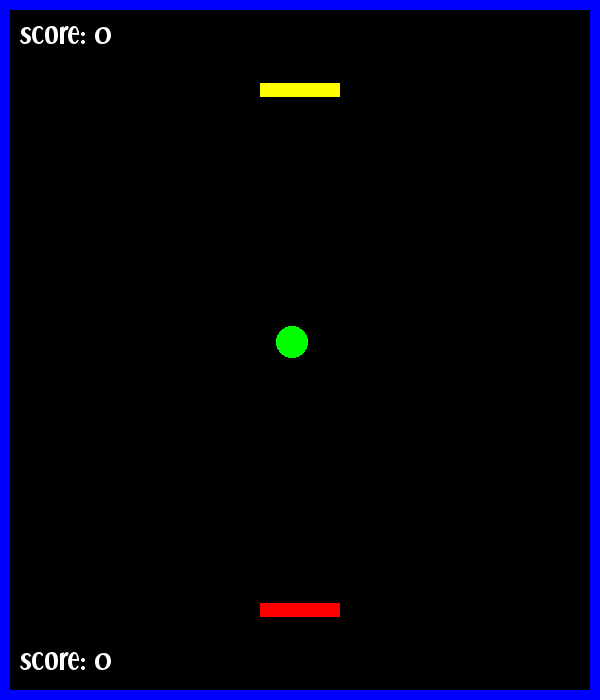
\includegraphics[width=0.5\textwidth]{game_screen.png}
\caption{Interfejs graficzny gry}
\label{fig:game}
\end{figure}

Sterowanie może odbywać się przy pomocy myszki lub kamery. Jeśli użytkownik wybierze opcję sterowania przy pomocy kamery wykorzystujemy bibliotekę OpenTLD,
która ułatwia śledzenie obiektów (opis użytego algorytmu znajduje się w sekcji~\ref{TLD}).\footnote{Bilioteka OpenTLD udostępniana jest na licencji GNU General Public License}

\subsection{Zasady gry}

Gra jest prostą symulacją tenisa stołowego w dwóch wymiarach. Od bocznych ścian piłka odbija się, natomiast jeśli jeden z graczy nie zdoła jej odbić odpowienio na dole lub górze
planszy to przeciwnik zdobywa punkt. Celem gry jest zdobycie większej ilości punktów od przeciwnika.\footnote{Szczegółowy opis zasad i historia gry znajduje się na \emph{http://en.wikipedia.org/wiki/Pong}}

\subsection{Konfiguracja kamery}

Jeśli wybierze się opcję sterowania z użyciem kamery pojawia się dodatkowe okno z widokiem z kamery.
Okno umożliwia konfigurację programu. Aby możliwe było sterowanie platformą konieczne jest zaznaczenie przedmiotu który ma być śledzony.

\begin{tightlist}
\item \keystroke{r} -- wyczyść obecne zaznaczenie i rozpocznij zbieranie nowego zaznaczenia
\item \keystroke{space} -- rozpocznij grę
\item \keystroke{q} lub \keystroke{escape} -- wyjdź
\end{tightlist}

\subsection{Sterowanie przy pomocy myszki}

W przypadku sterowania z użyciem myszki platformą steruje się poprzez ruch myszki nad oknem z grą.

\begin{tightlist}
\item \keystroke{mouse} -- poruszanie platformą
\item \keystroke{space} -- rozpocznij grę
\item \keystroke{escape} -- wyjdź
\end{tightlist}

\section{Podjęte próby rozwiazania}

Cały projekt możemy z pewnością potraktować jako duży poligon doświadczalny w zakresie przetwarzania obrazu. Zanim zastosowaliśmy algorytm TLD próbowaliśmy dwóch innych sposobów:

\begin{tightlist}
\item autorskie rozwiązanie w oparciu o próbkowanie koloru
\item rozwiązanie oparte na algorytmie CAMShift
\end{tightlist}

\subsection{Autorskie rozwiązanie}

Autorskie rozwiązanie składało się z 2 kroków konfiguracji:

\begin{tightlist}
\item zaznaczenie obszaru który chcemy śledzić
\item dobór odpowiednich wartości HSV
\end{tightlist}

Po zaznaczeniu obszaru nasz algorytm obliczał średnie wartości HSV dla zaznaczonego obszaru. Następnie wyświetlał użytkownikowi otrzymane wartości w celu ręcznego ich dopasowania (na bazie otrzymanych wartości tworzył przedziały). Algorytm dobrze radził sobie z charakterystycznymi kolorami (np. zielonym markerem). Napotkaliśmy jednak trzy problemy:

\begin{tightlist}
\item po początkowej kalibracji zmiany oświetlenia uniemożliwiały płynną grę
\item w przypadku zgubienia ręki występowały trudności z jej ponownym odnalezieniem
\item mylenie dłoni z głową
\end{tightlist}

Ponieważ charakter naszej aplikacji wymagał braku skokowości (nie mogliśmy sobie pozwolić na choćby chwilowe zgubienie pozycji dłoni) powyższy algorytm nie sprawdził się w przypadku sterowania ciałem. Sprawdziłby się w przypadku użycia odpowiedniego markera.

\subsection{Camshift}

Kolejną próbą był algorytm CAMShift. Algorytm zachowywał się znacznie lepiej jeśli chodzi o ciągłość pomiarów (rzadko zdarzały się sytuacje w których program gubił dłoń). Odbywało się to jednak tylko w przypadku spełnienia odpowiednich założeń:

\begin{tightlist}
\item{ tylko ręka jest przed ekranem (brak głowy) }
\item{ w miarę odizolowane tło}
\end{tightlist}

Niestety również ten algorytm nie nadał się jako finalne rozwiązanie. Uznaliśmy, że przyjemność czerpana z gry jest zbyt niska. Wynikało to głównie z faktów że:

\begin{tightlist}
\item{algorytm miał spore problemy z wykryciem ponownie dłoni gdy ta opuściła ekran}
\item{płynna gra wymagała zbyt dużych naszym zdaniem założeń (czyste tło, brak głowy w kamerze)}
\end{tightlist}

Z powodu wysoko postawionych założeń jeśli chodzi o przyjemność grania odrzuciliśmy również to rozwiązanie.

\section{Opis algorytmu TLD} \label{TLD}

Zadaniem algorytmu jest śledzenie bieżącej pozycji danego obiektu w kolejnych klatkach pobranych z kamery. Jest on pół-automatyczny -- wymaga początkowego zaznaczenia obiektu przez użytkownika.
Działanie algorytmu oparte jest na rekurencyjnym śledzeniu (przewidywaniu nowej pozycji na podstawie wcześniejszych)
oraz na wykrywaniu obrazów podobnych do szablonów dostosowanych do jasności i wielkości.
Podstawą detektora są znalezione szablony zarówno pasujące jak i nie pasujące. Jeśli detektor odnajdzie z dużym podobieństwem pasujący szablon,
rekurencyjne śledzenie jest reinicjalizowane w tym miejscu. \\

Powyższe rozwiązanie łączy stosunkowo krótki czas wykonania z dobrą efektywnością. Rozwiązuje następujące problemy:

\begin{tightlist}
\item odróżnianie śledzonego obiektu od innych podobnych do niego
\item śledzenie obiektów które zniknęły (schowały się za czymś lub wyszły poza obraz z kamery) i powróciły
\item rozpoznawanie lekko zmodyfikowanych obiektów -- obróconych, przybliżonych lub oddalonych od kamery
\item czas wykonania -- bardzo ważny w przypadku sterowania grą
\end{tightlist}

\begin{figure}[!ht]
\centering
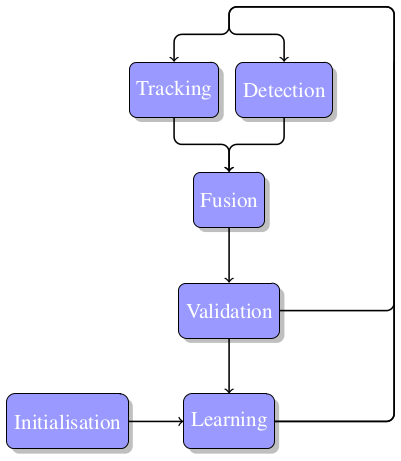
\includegraphics[width=0.5\textwidth]{alg_flow.png}
\caption{Przepływ działania algorytmu. Pochodzi z~\cite{TLD-thesis}.}
\label{fig:flow}
\end{figure}

Algorytm został szczegółowo opisany w~\cite{TLD-thesis}.

\section{Wyniki} \label{results}

\begin{figure}[!ht]
\centering
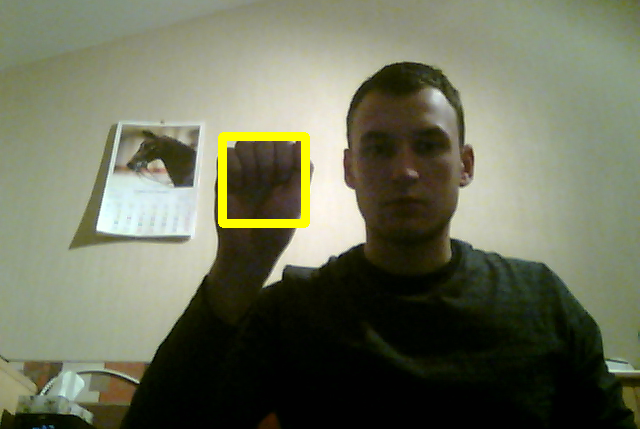
\includegraphics[width=0.5\textwidth]{fist-yellow.png}
\caption{Śledzenie pięści -- kolor żółty oznacza uczenie.}
\label{fig:fist-yellow}
\end{figure}

Najlepsze wyniki udało nam się uzyskać podczas śledzenia zaciśniętej pięści i głowy.
Trzeba mieć na uwadze, że sterowanie głową jest nieprzyjemne i może szybko doprowadzić do zawrotów.
Przy dobrym oświetleniu pozycja jest rzadko gubiona, a co za tym idzie gra jest płynna.

\begin{figure}[!ht]
\centering
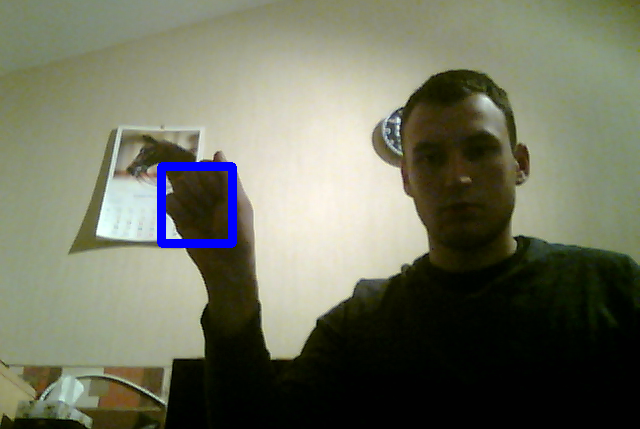
\includegraphics[width=0.5\textwidth]{fist-blue.png}
\caption{Śledzenie pięści -- kolor niebieski oznacza stabilny obraz.}
\label{fig:fist-blue}
\end{figure}

Śledzenie otwartej dłoni daje gorsze wyniki, jedynie przy bardzo dobrym oświetleniu
i braku innych obiektów o podobnym kształcie i kolorze śledzenie jest płynne. \\

Należy pamiętać, że gra z wykorzystaniem gestów sprawia największą przyjemność wtedy,
gdy przeciwnik również korzysta z tej opcji.
Sterowanie przy pomocy myszki wciąż pozostaje najbardziej precyzyjne.

\begin{figure}[!ht]
\centering
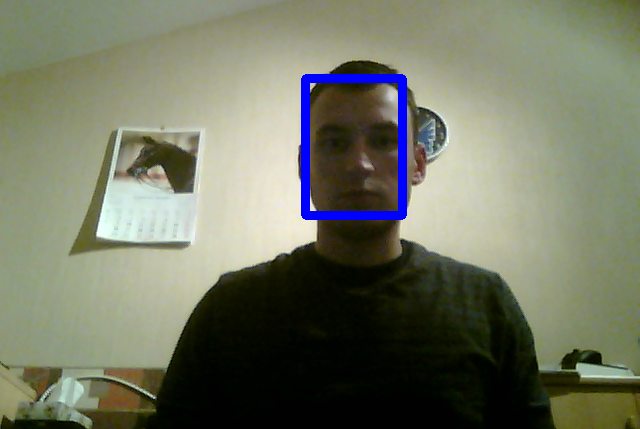
\includegraphics[width=0.5\textwidth]{head-blue.png}
\caption{Śledzenie głowy daje najlepsze wyniki ale nie sprzyja graniu.}
\label{fig:head-blue}
\end{figure}

\begin{thebibliography}{9}

\bibitem{TLD-thesis}
  Georg Nebehay,
  \emph{Robust Object Tracking Based on Tracking-Learning-Detection}.
  Uniwersytet Techniczny, Wiedeń,
  2012.

\end{thebibliography}

\end{document}
